% Created 2025-01-14 Tue 20:16
% Intended LaTeX compiler: pdflatex
\documentclass[presentation]{beamer}
\usepackage[utf8]{inputenc}
\usepackage[T1]{fontenc}
\usepackage{graphicx}
\usepackage{longtable}
\usepackage{wrapfig}
\usepackage{rotating}
\usepackage[normalem]{ulem}
\usepackage{amsmath}
\usepackage{amssymb}
\usepackage{capt-of}
\usepackage{hyperref}
\nocite{*}
\usepackage[T1]{fontenc}
\usepackage[utf8]{inputenc}
\usepackage[spanish]{babel}
\usepackage[backend=biber, style=apa]{biblatex}
\addbibresource{/home/richi20/Tareas/Presebtacion_Grupal/ExposicionArqui/bibliography.bib}
\usetheme{default}
\usecolortheme{}
\usefonttheme{}
\useinnertheme{}
\useoutertheme{}
\author{Lenin G. Falconí, Richard Dawkins, Richard Tipantiza}
\date{}
\title{S9-Memoria-del-Sistema}

\hypersetup{
 pdfauthor={Lenin G. Falconí, Richard Dawkins, Richard Tipantiza},
 pdftitle={S9-Memoria-del-Sistema},
 pdfkeywords={},
 pdfsubject={},
 pdfcreator={Emacs 27.1 (Org mode 9.3)}, 
 pdflang={Spanish}}
\begin{document}

\maketitle
\begin{frame}{Outline}
\tableofcontents
\end{frame}



\section{Indicaciones}
\label{sec:orgc69a0f2}
\begin{frame}[allowframebreaks]{Indicaciones}
\end{frame}
\begin{frame}[label={sec:orgcd70fcc}]{Diseño de las Diapositivas}
\begin{itemize}
\item Para diseñar sus diapositivas puede consultar cualquiera de las
presentaciones .ORG desarrolladas por el profesor así como al
archivo \href{https://github.com/LeninGF/EPN-Lectures/blob/main/iccd332ArqComp-2024-B/Tutoriales/Beamer-Emacs/tutorialBeamer.org}{tutorialBeamer.org} en el repositorio de \href{https://github.com/LeninGF/EPN-Lectures/blob/main/iccd332ArqComp-2024-B/Tutoriales/Beamer-Emacs/tutorialBeamer.org}{GitHub} de la clase.
\item Recuerde que los archivos .ORG son archivos de texto así que los
puede copiar y sustituir por su texto propio.
\end{itemize}
\end{frame}
\begin{frame}[label={sec:org00a1a00}]{Sobre este Documento}
\begin{itemize}
\item Este documento tiene la propuesta de temas a tratar y desarrollar
por los estudiantes.
\item Se ha de utilizar como base la bibliografía recomendada, pero puede
consultar bibliografía adicional.
\end{itemize}
\end{frame}
\section{Memoria Cache (E2, 11, 162)}
\label{sec:org1aeb46c}
\begin{frame}[label={sec:org4824df3}]{Principios Básicos de las Memorias Caché (E2,11,163)(E2,7,133)}
\alert{\alert{\alert{¿Para que sirve?}}} 


El objetivo principal de la memoria caché es mejorar la velocidad de acceso a los datos almacenados, combinando el acceso rápido a datos de una memoria más cara y de alta velocidad (memoria caché) con el almacenamiento más lento pero de mayor capacidad de la memoria principal.


\alert{\alert{\alert{Funcionamiento}}}


\begin{itemize}
\item La CPU transfiere palabras o bloques entre la caché y la memoria principal. La caché actúa como intermediaria rápida entre la CPU y la memoria principal, almacenando temporalmente datos que la CPU necesita frecuentemente.
\end{itemize}
\end{frame}


\begin{frame}[label={sec:org374099d}]{Principios Básicos de las Memorias Caché (E2,11,163)(E2,7,133)}
\begin{itemize}
\item En el modelo simple de caché (como muestra la Figura 5.1a), la CPU realiza transferencias rápidas a la caché y transferencias más lentas a la memoria principal.
\end{itemize}

\begin{center}
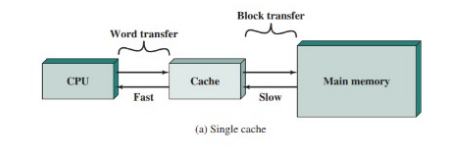
\includegraphics[width=.9\linewidth]{./Imagenes/captura1.png}
\end{center}
\end{frame}

\begin{frame}[label={sec:orge6152e4}]{Principios Básicos de las Memorias Caché (E2,11,163)(E2,7,133)}
Niveles de Caché: Se organizan en varios niveles (L1, L2, L3). A medida que se avanza en los niveles, la velocidad disminuye, pero la capacidad aumenta.

\begin{itemize}
\item Caché de Nivel 1 (L1): La más rápida y de menor capacidad.
\item Caché de Nivel 2 (L2): Un poco más lenta, pero con mayor capacidad.
\item Caché de Nivel 3 (L3): Menos rápida que L1 y L2, pero aún más rápida que la memoria principal.
\end{itemize}


\begin{block}{Elementos de Diseño de la memoria Caché}
\end{block}
\begin{block}{Introducción a la Caché}
\begin{itemize}
\item "La memoria caché mejora la velocidad de acceso
al reducir la distancia entre el procesador y la memoria principal."
\item "Los fallos de caché generan tráfico en el bus del sistema."
\end{itemize}
\begin{center}
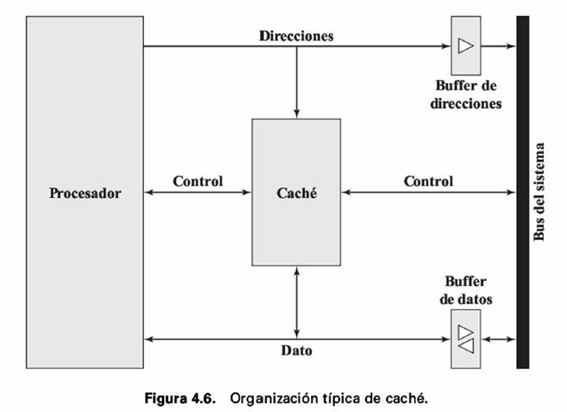
\includegraphics[width=.9\linewidth]{./Imagenes/fig4.6.png}
\end{center}
\end{block}
\begin{block}{Parámetros de Diseño de la Caché}
\begin{itemize}
\item "La función de correspondencia, el tamaño de línea y el algoritmo de sustitución
son clave para el diseño de una caché eficiente."
\item "La jerarquía de cachés puede mejorar el rendimiento en aplicaciones bien optimizadas."
\begin{center}
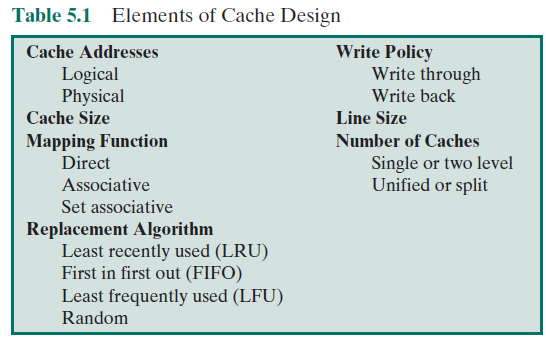
\includegraphics[width=.9\linewidth]{./Imagenes/tabla5.1.png}
\end{center}
\end{itemize}
\end{block}


\begin{block}{Tamaño Caché}
\begin{itemize}
\item "El tamaño de la caché impacta directamente en su velocidad y costo."
\item "No existe un tamaño 'óptimo' único, ya que depende de la naturaleza de las tareas."
\begin{center}
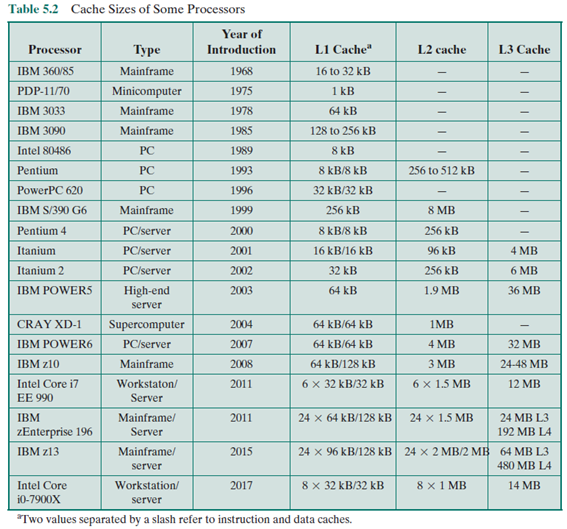
\includegraphics[width=.9\linewidth]{./Imagenes/tabla5.2.png}
\end{center}
\end{itemize}
\end{block}

\begin{block}{Tipos de caché}
\begin{itemize}
\item "La caché lógica utiliza direcciones virtuales; la física, direcciones físicas."
\item "La caché lógica puede ser más rápida pero requiere mayor gestión en cambios de contexto."
\begin{center}
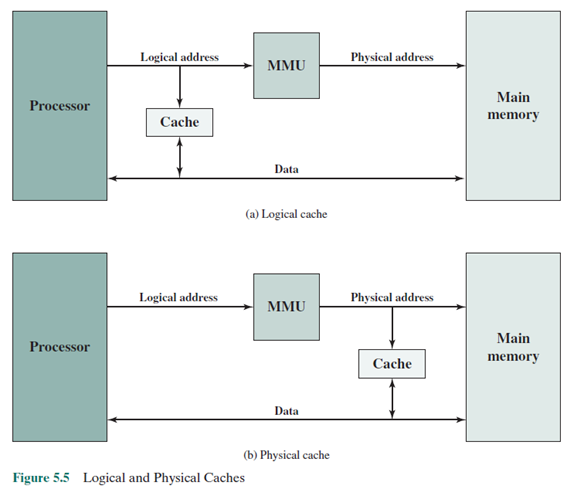
\includegraphics[width=.9\linewidth]{./Imagenes/fig5.png}
\end{center}
\end{itemize}
\end{block}
\end{frame}




\begin{frame}[label={sec:org3b03b5a}]{Función de Correspondencia (E2,11,170)(E2,7,137)}
\begin{itemize}
\item Se recomienda la tabla 5.3 página 170 de la 10ma edición
\end{itemize}
\end{frame}

\section{Algoritmo de Sustitución}
\label{sec:orgd459187}
\begin{frame}[allowframebreaks]{Algoritmo de Sustitución (E2,7,148)}
Una vez llena la caché, se debe reemplazar un bloque existente para introducir uno nuevo.
En correspondencia directa, no hay elección, ya que cada bloque tiene una línea específica.
En técnicas asociativas, se requieren algoritmos de sustitución implementados en hardware para alta velocidad.\autocite{stallings2006organización}
\begin{enumerate}
\item LRU (Least Recently Used)
\item FIFO (First-In-First-Out
\item LFU (Least Frequently Used
\item Aleatoria
\end{enumerate}
\end{frame}

\section{Política de escritura}
\label{sec:org4b31c5e}
\begin{frame}[allowframebreaks]{Política de escritura}
\begin{itemize}
\item Casos de reemplazo en caché
\begin{enumerate}
\item Casos de reemplazo en caché
\item Casos de reemplazo en caché
\end{enumerate}
\item Problemas al reemplazar bloques
\begin{enumerate}
\item Acceso múltiple a la memoria principal
\item Sistemas multiprocesado
\end{enumerate}
\item Sistemas multiprocesado
\begin{enumerate}
\item Escritura inmediata
\item Postescritura
\end{enumerate}
\item Estadísticas de escritura
\item Vigilancia del bus con escritura inmediata
\item Transparencia hardware
\item Memoria excluida de caché
\end{itemize}
\end{frame}

\section{Tamaño de Linea}
\label{sec:org37f9158}
\begin{frame}[allowframebreaks]{Tamaño de Línea}
\begin{itemize}
\item Tamaño de línea de caché:
\item Efectos al aumentar el tamaño del bloque:
\begin{enumerate}
\item Reducción de bloques en caché
\item Mayor distancia de las palabras adicionales:
\end{enumerate}
\item Relación compleja entre tamaño y tasa de aciertos
\end{itemize}
\end{frame}
\begin{frame}[label={sec:org7600033}]{Número de Cachés (E2, 7, 150)}
\end{frame}


\section{Referencias}
\label{sec:orgb7127eb}
\begin{frame}[allowframebreaks]{Bibliografía}
\printbibliography
\end{frame}
\end{document}
